\section{Literature Review: Fragmented Recognition and Systematic Blindness}

\subsection{The Peripheral Scouts}

A careful survey of contemporary scholarship reveals a curious phenomenon: researchers at the edges of multiple disciplines have independently begun recognizing the energetic dimensions of cognition, yet these insights remain unintegrated, failing to coalesce into a unified framework that could challenge the dominant paradigm of costless information processing.

In management science, \citet{bratianu2020} claims to use ``for the first time a thermodynamics approach'' to understand knowledge dynamics, proposing knowledge entropy as an organizing principle for organizational cognition. That such a claim could be made in 2020 (decades after information theory established entropy measures) reveals the profound isolation between knowledge management and physical sciences. \citet{bratianu2020b} extend this framework, arguing that knowledge manifests in three forms (rational, emotional, spiritual) that transform through ``energy-like processes,'' yet they stop short of recognizing that these are not metaphorical but literal energy transformations.

In neuroscience, researchers have begun quantifying the metabolic costs of cognition with increasing precision. \citet{jamadar2025} demonstrates that goal-directed cognition requires only 5\% more energy than resting brain activity: a finding that paradoxically reveals both the brain's efficiency and the critical importance of that marginal energy investment. \citet{wiehler2022} provide mechanistic evidence that cognitive control exertion leads to glutamate accumulation in the lateral prefrontal cortex, establishing a direct biochemical basis for mental fatigue. These findings suggest that ``cognitive work'' is not merely analogous to physical labor but operates through similar energetic constraints.

The 5\% additional energy investment represents not cognitive work itself but focused execution: the "sprint" of deliberate concentration required to capture, refine, and formalize what emerged during seemingly idle processing. \citet{wiehler2022} provide mechanistic evidence that this cognitive control exertion leads to glutamate accumulation in the lateral prefrontal cortex, establishing a direct biochemical basis for mental fatigue from sustained focus. The energetic constraint is real—but it operates on both the generative baseline and the refinement sprint.

These findings reveal that cognitive work is not merely analogous to physical labor but operates through similar energetic constraints with a critical distinction: the most valuable cognitive processes—those generating novel insights, cross-domain synthesis, and adaptive responses—occur during what measurement systems dismiss as "unproductive" time. Educational systems and organizations optimizing for measurable outputs systematically eliminate the energetically expensive baseline processing that generates genuine understanding, preserving only the 5\% sprint of formalization while starving the 95\% foundation that makes formalization worthwhile.

In physics and information theory, \citet{stonier1996} proposed treating information as a basic property of the universe alongside matter and energy, arguing for fundamental interconvertibility between information and energy. Yet this theoretical breakthrough remains largely unknown to knowledge management scholars, who continue treating information as an abstract, costless commodity.

\subsection{The Mainstream Blindness: The SECI Delusion and the Energy Void}

Despite peripheral recognition of cognitive energetics, the dominant discourse in knowledge management, organizational theory, and educational policy proceeds as if cognition were thermodynamically neutral. The vast literature on the ``knowledge economy'' \citep{powell2004knowledge}, ``learning organizations'' \citep{senge1990}, and ``competency-based education'' \citep{mulder2007competency} treats knowledge as an infinitely reproducible resource constrained only by access and transmission bandwidth---never by the metabolic energy required to create, maintain, and transform it.

\subsubsection{The SECI Model: Thermodynamics Hidden in Plain Sight}

The most reproduced image in knowledge management literature may also be its most deceptive. \citeauthor{nonaka1995knowledge}'s (\citeyear{nonaka1995knowledge}) SECI model---cited over 30,000 times---presents knowledge creation as an elegant spiral flowing through four transformation modes: Socialization $\rightarrow$ Externalization $\rightarrow$ Combination $\rightarrow$ Internalization. The diagram shows smooth movement between quadrants, spiraling upward toward organizational wisdom. It is elegant, intuitive, and taught in every business school.

What it systematically obscures is the energy required for that movement.

\paragraph{The Orthodox Delusion Meets Thermodynamic Reality}

Figure~\ref{fig:seci-comparison} presents the SECI Knowledge Creation Model in its orthodox representation alongside the thermodynamic reality. The contrast reveals what 30,000 citations have systematically obscured.

\begin{figure}[htbp]
\centering
\begin{subfigure}[b]{0.48\textwidth}
    \centering
    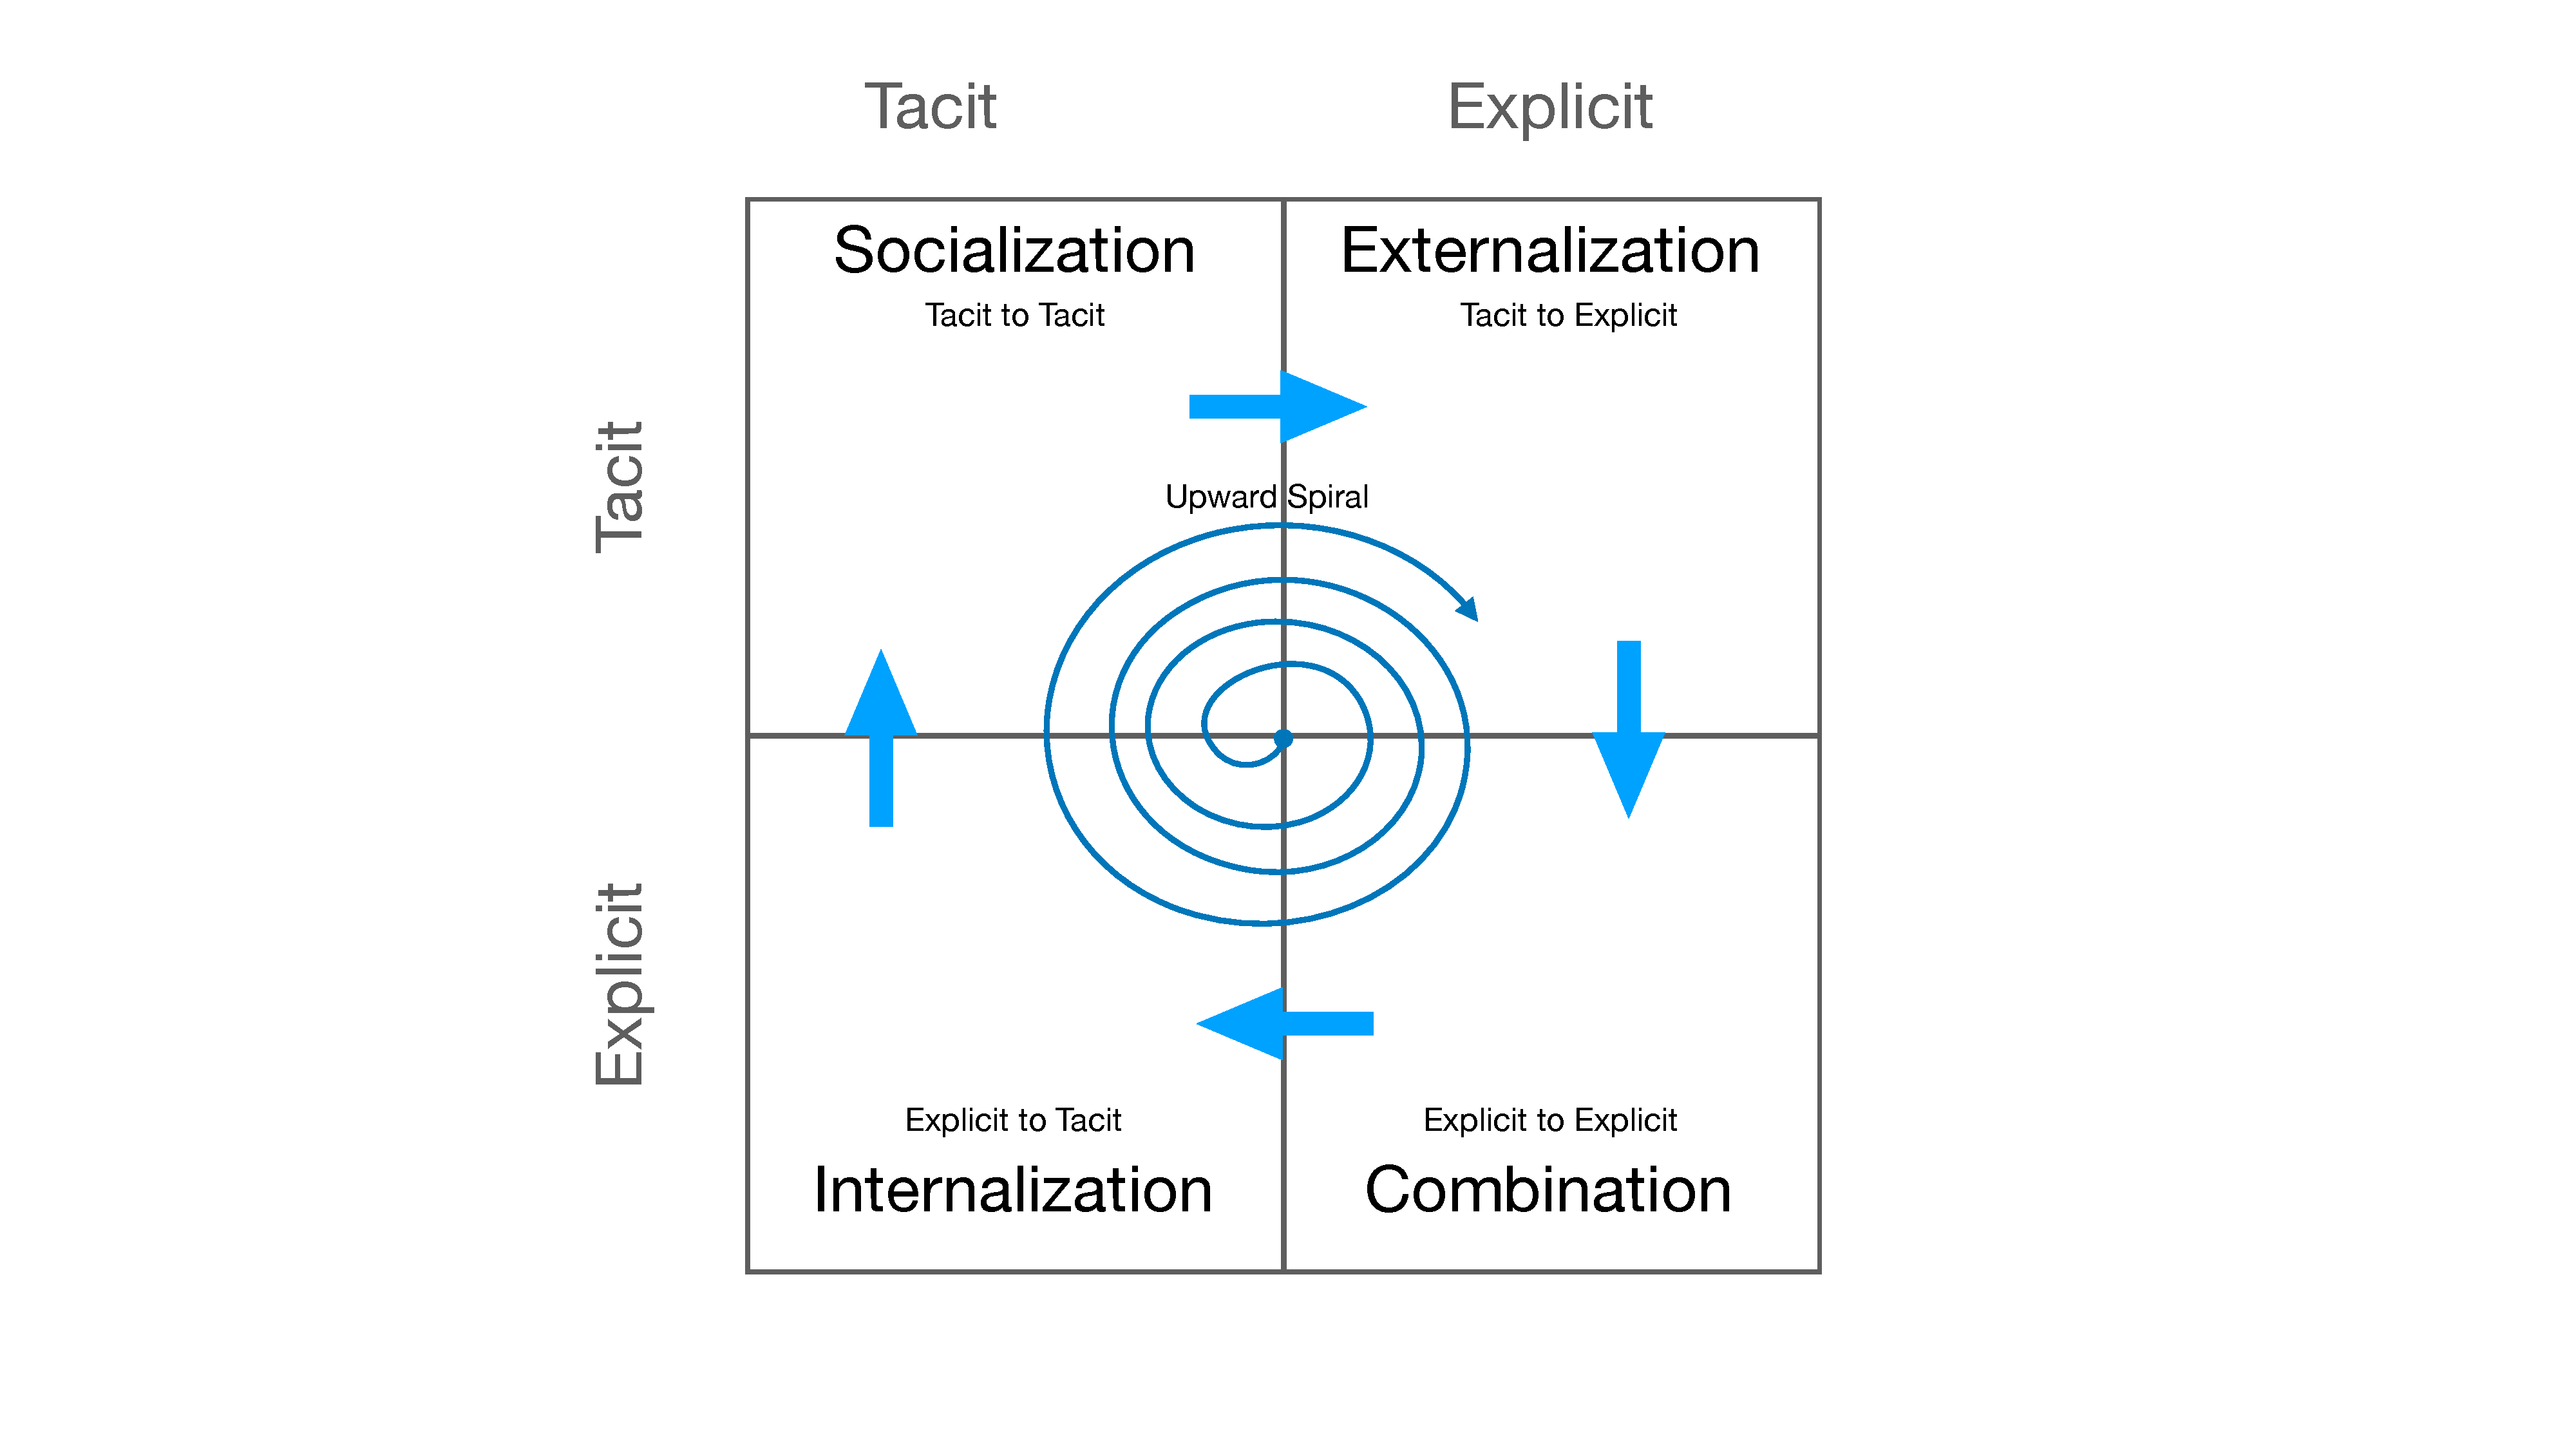
\includegraphics[width=\textwidth]{../figures/seci-orthodox}
    \caption{Orthodox Representation}
    \label{fig:seci-orthodox}
\end{subfigure}
\hfill
\begin{subfigure}[b]{0.48\textwidth}
    \centering
    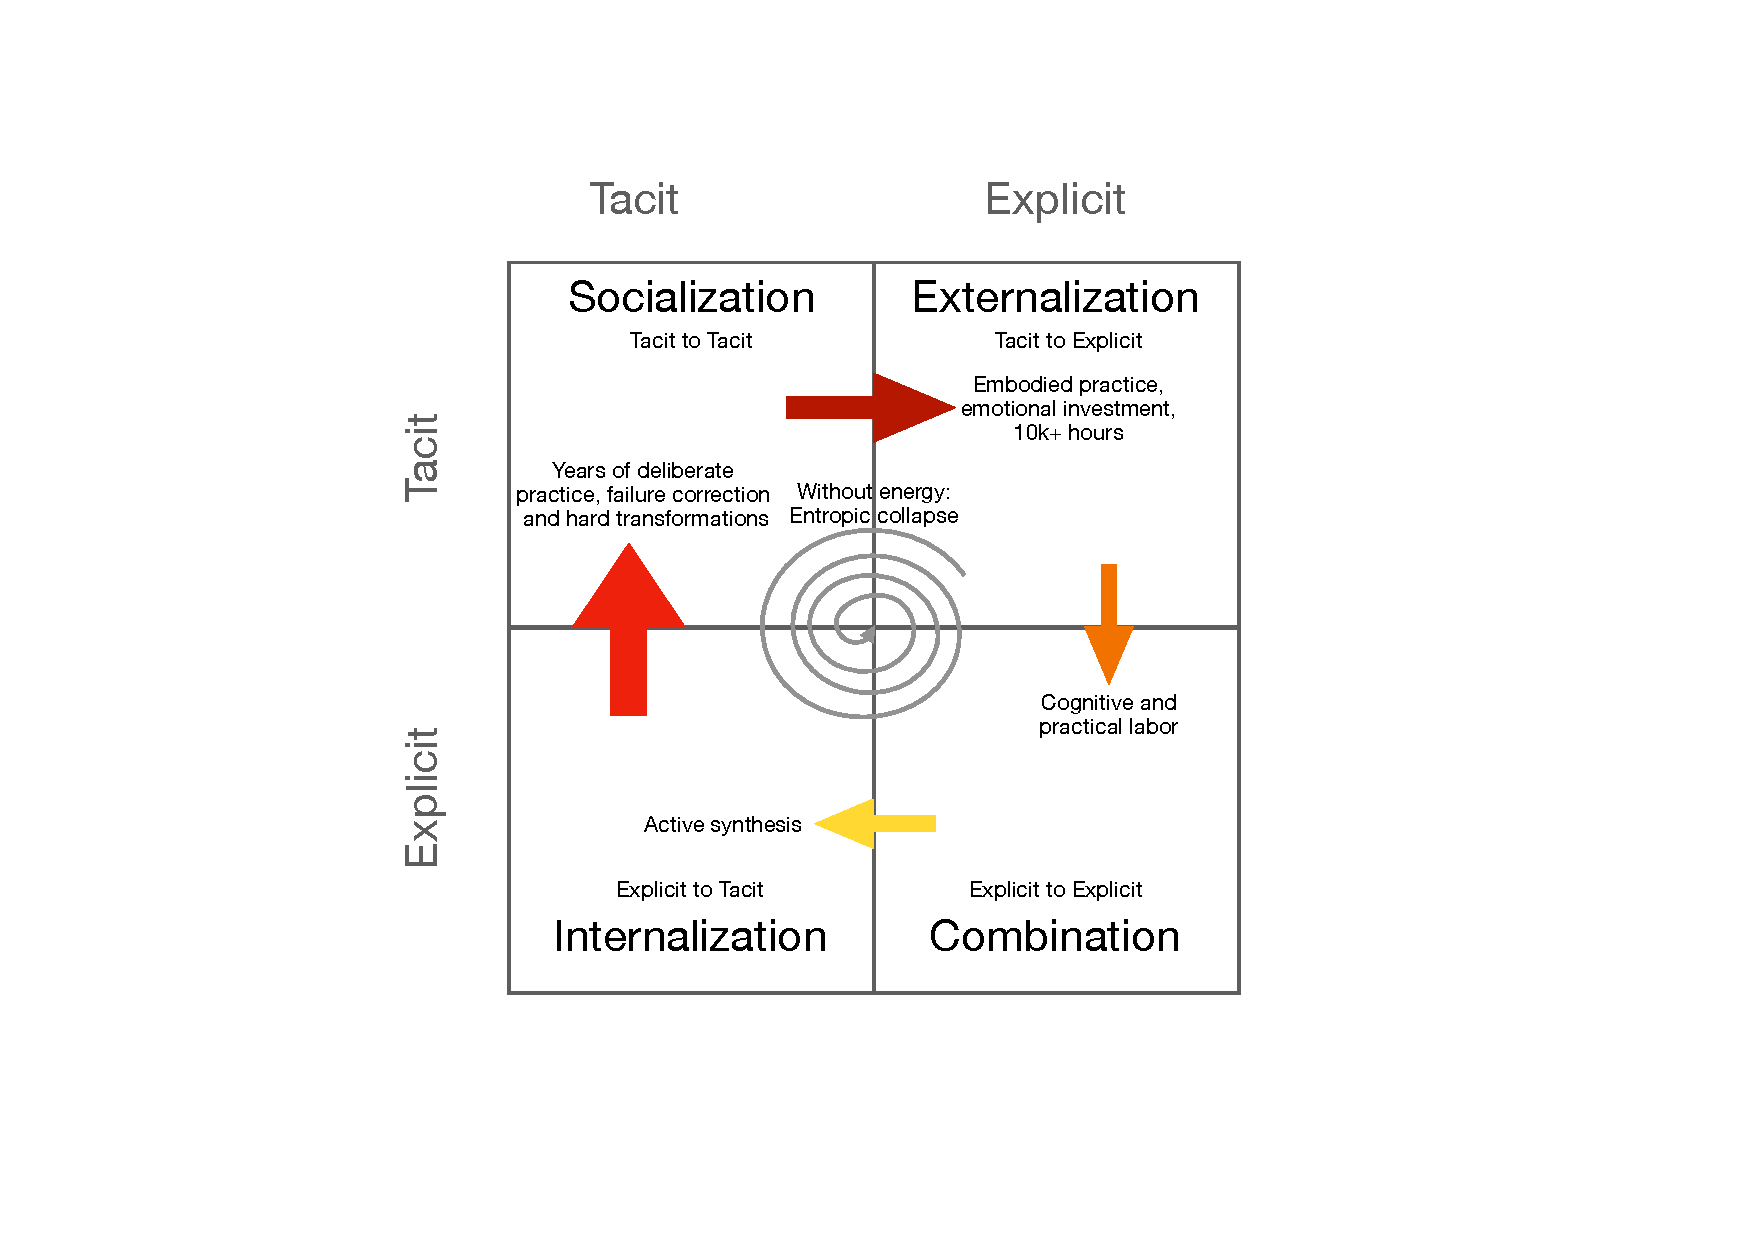
\includegraphics[width=\textwidth]{../figures/seci-thermodynamic}
    \caption{Thermodynamic Reality}
    \label{fig:seci-thermodynamic}
\end{subfigure}
\caption{The SECI Knowledge Creation Model: Orthodox vs. Thermodynamic Perspectives. (a) The standard depiction shows knowledge transforming smoothly through four modes: Socialization (tacit-to-tacit), Externalization (tacit-to-explicit), Combination (explicit-to-explicit), and Internalization (explicit-to-tacit). Arrow uniformity implies equivalent ease across all transformations. The spiral suggests self-sustaining upward momentum. Energy requirements remain invisible. (b) The same model with energy investments visible. Arrow thickness represents magnitude of required investment: Socialization (10,000+ hours of apprenticeship); Externalization (high cognitive labor plus 30--70\% information degradation); Combination (sustained 5\% above baseline metabolic cost); Internalization (months-to-years of deliberate practice). The spiral no longer appears self-sustaining but requires continuous energy investment exceeding entropic losses at each transformation.}
\label{fig:seci-comparison}
\end{figure}

The orthodox representation (Figure~\ref{fig:seci-orthodox}) has achieved near-universal acceptance precisely because it makes knowledge management appear achievable through organizational design alone. Document the tacit, combine the explicit, socialize the workforce, internalize the procedures---the spiral will naturally ascend. Thirty thousand citations later, organizations worldwide have implemented SECI frameworks while systematically disinvesting in the energy that makes transformation possible.

The thermodynamic view (Figure~\ref{fig:seci-thermodynamic}) reveals why these implementations fail with such predictable regularity. Each transformation mode demands specific energy investments that organizations systematically refuse to provide:

\textbf{Socialization} (Tacit $\rightarrow$ Tacit): The thickest arrow. Master craftspeople develop embodied knowledge through 10,000+ hours of practice---Ericsson's deliberate practice threshold \citep{ericsson1993}. Medieval guilds required 7--10 year apprenticeships not from tradition but from thermodynamic necessity: the time needed to build neural architectures capable of intuitive expertise. Contemporary organizations replacing apprenticeships with onboarding sessions attempt to transfer decades of accumulated negentropy through PowerPoint presentations. The energy investment: 10,000+ hours minimum. The organizational allocation: typically 40--80 hours. The gap: thermodynamic impossibility.

\textbf{Externalization} (Tacit $\rightarrow$ Explicit): The double-line arrow indicating high friction. Polanyi's insight that ``we know more than we can tell'' \citep{polanyi1966} isn't philosophical mystery but thermodynamic reality. Tacit knowledge exists as high-dimensional neural network states---millions of weighted connections developed through practice. Externalizing this into linear text or explicit procedures requires intensive cognitive labor (sustained attention, memory reconstruction, language translation) plus acceptance of massive information loss: 30--70\% fidelity degradation is typical \citep{collins2010}. Organizations demanding rapid documentation while eliminating reflection time guarantee low-fidelity extraction. The expert surgeon's embodied knowledge of tissue resistance becomes the procedure manual's ``apply appropriate pressure.'' The energy investment: High cognitive labor sustained over weeks/months. The organizational allocation: ``document your process by Friday.'' The result: entropic decay masquerading as knowledge capture.

\textbf{Combination} (Explicit $\rightarrow$ Explicit): The deceptively modest arrow. Combining documented knowledge appears algorithmic---merge databases, cross-reference procedures, synthesize reports. Yet genuine synthesis (not mere aggregation) requires the 5\% above-baseline metabolic cost that \citet{jamadar2025} measured. Maintaining focus for hours while identifying patterns, resolving contradictions, and generating insights demands sustained cognitive energy. Organizations automating combination through software eliminate the human energy investment that distinguishes synthesis from compilation. The energy investment: Sustained 5\% metabolic premium over hours/days. The organizational allocation: ``Let the system integrate the data.'' The gap: humans thinking versus algorithms sorting.

\textbf{Internalization} (Explicit $\rightarrow$ Tacit): Another thick arrow. Reading procedures doesn't create competence---practice does. Converting explicit knowledge into embodied capability requires months-to-years of deliberate practice with feedback loops. Motor skills, perceptual discrimination, intuitive pattern recognition---all demand sustained energy investment building neural infrastructure. Organizations eliminating practice time while expecting documented procedures to become embodied expertise are attempting thermodynamic impossibility. The thick arrow in Figure~\ref{fig:seci-thermodynamic} represents years of energy investment---energy that micro-credentialing and competency-based education systematically refuse to provide.

\paragraph{The Spiral That Cannot Rise}

The SECI model's most dangerous fiction is the upward spiral itself. \citeauthor{nonaka1995knowledge} show knowledge spiraling higher through repeated cycles---individual tacit becomes group tacit becomes organizational explicit becomes individual internalized becomes group socialized at higher level, ascending continuously toward organizational wisdom.

But entropy pulls downward. Every transformation loses energy to heat. Every externalization degrades fidelity. Every combination without genuine synthesis merely shuffles information. Every internalization without adequate practice hours creates credential illusion rather than capability. The spiral rises only when energy input exceeds entropic loss at each transformation.

Organizations implementing SECI frameworks while simultaneously reducing training time (less socialization energy), demanding faster documentation (less externalization care), automating synthesis (zero combination energy), and eliminating practice time (minimal internalization investment) are running the spiral in reverse. They are building entropy accelerators while calling them knowledge management systems.

\paragraph{The 30,000 Citation Blindness}

That this model achieved over 30,000 citations without anyone questioning the absence of energy accounting reveals our civilizational blind spot. We see elegant patterns and assume they're self-sustaining. We teach them in business schools as if transformation were costless. We implement them in organizations as if documentation were knowledge.

Nonaka himself approached recognition of the problem in his later concept of ``\textit{ba}''---the shared context providing foundation for knowledge creation \citep{nonaka1998ba}. But he frames it as philosophical space rather than literal metabolic investment. The energy remains invisible, therefore unbudgeted, unmeasured, and systematically disinvested. Organizations following the SECI model wonder why their spirals collapse. The answer is thermodynamics: the Second Law doesn't care about our elegant diagrams.

\subsubsection{The Broader Pattern of Energy Blindness}

The SECI model exemplifies a pattern pervading knowledge management literature. \citeauthor{senge1990}'s (\citeyear{senge1990}) ``learning organizations'' celebrate continuous learning without accounting for the energy required to sustain it. \citet{powell2004knowledge} analyze the ``knowledge economy'' without recognizing that knowledge represents high-energy states requiring investment to maintain. \citet{mulder2007competency} promote ``competency-based education'' that fragments learning into discrete assessments while eliminating the sustained practice necessary for genuine competence development.

Similarly, the burgeoning literature on artificial intelligence and knowledge work---from \citeauthor{brynjolfsson2014second}'s (\citeyear{brynjolfsson2014second}) ``Second Machine Age'' to \citeauthor{susskind2020future}'s (\citeyear{susskind2020future}) ``Future of the Professions''---focuses on computational capability and pattern recognition while ignoring the energetic basis that distinguishes biological from silicon cognition. These works treat the replacement of human expertise as a matter of algorithmic sophistication rather than recognizing it as the logical endpoint of a century-long process of cognitive energy disinvestment.

We trained humans to process knowledge through standardized, modular, assessable transformations---exactly the SECI quadrants but with minimal energy investment. We documented these energy-depleted processes exhaustively. Then we built AI systems that learned from our documentation. The machines succeed at replacing human expertise not because they've achieved human capability but because we've reduced human capability to what machines can replicate: low-energy pattern processing divorced from the metabolic investments that once made expertise irreplaceable.

The mainstream literature proceeds as if knowledge were costless information rather than expensive biology. This blindness isn't accidental but structural---a consequence of disciplinary boundaries that separate thermodynamics from cognition, physics from knowledge management, energy from information. The SECI model with 30,000 citations but zero energy accounting stands as monument to our systematic refusal to acknowledge what physics makes unavoidable: knowledge creation requires continuous energy investment against entropy, and every optimization that reduces that investment accelerates the collapse it claims to prevent.

\subsection{Cognitive Capitalism's Energy Blindness}

The critical literature on ``cognitive capitalism'' \citep{moulierboutang2007, vercellone2007} comes closest to recognizing the exploitation of mental resources yet still fails to ground this in thermodynamic reality. Moulier-Boutang distinguishes between ``labor-power'' (physical energy expenditure) and ``invention-power'' (cognitive functions) without recognizing that invention-power also requires literal energy investment: not metaphorical ``mental energy'' but actual glucose metabolism, ATP consumption, and entropic heat dissipation.

This blindness extends to the platform economy literature. \citet{zuboff2019} ``surveillance capitalism'' brilliantly exposes behavioral data extraction but doesn't recognize that platforms are essentially entropy accelerators, harvesting the organized complexity of human cognition while investing nothing in its maintenance or development. \citet{srnicek2017} ``platform capitalism'' identifies data as the new oil but misses that, unlike oil, cognitive resources require continuous energy investment to prevent degradation.

\subsection{The Expertise Literature Gap}

The extensive literature on expertise development (from \citet{ericsson2006} deliberate practice to \citet{kahneman2009} conditions for expert intuition) meticulously documents the time requirements for skill acquisition (the famous ``10,000 hours''), but rarely acknowledges these as energy investment requirements. When researchers note that expertise requires ``effort'' or ``cognitive load,'' they treat these as psychological rather than thermodynamic phenomena.

Even sophisticated critiques of expert systems, from \citet{dreyfus1979} to \citet{collins2010}, focus on the irreducibility of tacit knowledge without recognizing that this irreducibility stems from its high-energy state. Tacit knowledge resists formalization not because it is mysteriously ineffable but because maintaining it requires continuous metabolic investment that cannot be captured in static representations.

\subsection{The Integration Imperative}

What emerges from this review is not an absence of relevant insights but their tragic fragmentation. Neuroscientists measure metabolic costs without connecting to knowledge theory. Management scholars invoke entropy without thermodynamic grounding. Physicists theorize information-energy equivalence without application to human cognition. Critical theorists expose cognitive exploitation without energetic foundation.

This fragmentation is not accidental but structural: a consequence of disciplinary boundaries that mirror the very vectorization this paper critiques. Just as education has collapsed multidimensional cognition into specialized competencies, academia has partitioned the study of knowledge into non-communicating silos, preventing recognition of the unified thermodynamic reality underlying all cognitive phenomena.

The task before us is not to discover new facts but to synthesize existing insights into a framework that reveals what disciplinary fragmentation has hidden: the systematic transformation of high-energy spherical cognition into low-energy vectors suitable for algorithmic consumption, and the thermodynamic impossibility of maintaining cognitive sovereignty without corresponding energy investment.